\documentclass[12pt]{article}
\usepackage[margin=0.8in]{geometry}
\makeatletter
\renewcommand{\@maketitle}{\newpage\null\vskip -3.5em\begin{center}{\LARGE \@title \par}\end{center}\par\vskip 0.2em}
\makeatother
\usepackage{amsmath,amssymb}
\usepackage{booktabs}
\usepackage{graphicx}
\usepackage{hyperref}
\setlength{\parskip}{0.6em}
\setlength{\parindent}{0pt}

\title{Why the cut $x_{\mathbb P}<0.1$ is enough to subtract the $0n0n$ events}
\author{}
\date{}

\begin{document}
\maketitle

\section*{In short}

The $Xn$ selection removes \emph{all} coherent events, at any $x_{\mathbb P}$, so in principle we
should subtract all of them. But a coherent event at large $x_{\mathbb P}$ is almost impossible: the
nucleus has to absorb a minimum momentum $\sqrt{|t_{\min}|}\approx x_{\mathbb P}m_N$, and a large
nucleus can only take a very small kick without breaking up. Above $x_{\mathbb P}\approx0.05$ most
coherent events are forbidden, and at $x_{\mathbb P}=0.1$ only $5\%$ are left. So integrating up to
$x_{\mathbb P}=0.1$ already contains essentially all the coherent cross section, and going further
would not add physics.

\section*{1. What we have to subtract}

The inclusive calculation corresponds to the $An0n$ class: it includes every event, also those in
which the target nucleus stays intact (coherent diffraction). CMS measures $Xn0n$: it requires at
least one neutron from the target, so it throws away every event in which the target stays intact.
To compare with CMS we must subtract the coherent events.

This condition is about the \emph{nucleus}, not about a rapidity gap. CMS does not require a gap and
does not cut on $x_{\mathbb P}$. So the question is: which coherent events exist at all?

\section*{2. The nucleus must absorb a minimum momentum}

$x_{\mathbb P}$ is the fraction of the target momentum carried by the pomeron. The target (per
nucleon, mass $m_N$) therefore loses a fraction $x_{\mathbb P}$ of its longitudinal momentum,
$P'^-=(1-x_{\mathbb P})P^-$, and gets a transverse kick $\boldsymbol\Delta$. With both on shell,
the momentum transfer $t=(P-P')^2$ is (derivation in the Appendix)
\begin{equation}
  |t| = \frac{\boldsymbol\Delta^2 + x_{\mathbb P}^2m_N^2}{1-x_{\mathbb P}}
  \;\geq\; |t_{\min}| = \frac{x_{\mathbb P}^2m_N^2}{1-x_{\mathbb P}}\,.
\end{equation}
Even with no transverse kick, the target has to change its longitudinal momentum, so $|t|$ cannot
be zero. The larger $x_{\mathbb P}$, the larger the smallest possible kick:
$\sqrt{|t_{\min}|}\approx x_{\mathbb P}\,m_N$.

\section*{3. A large nucleus can only absorb a small kick}

In a coherent event, the photon scatters off the whole nucleus, which stays intact. The probability
for this is given by the nuclear form factor, $|F_A(t)|^2$, which is the Fourier transform of the
nuclear density. A nucleus of radius $R$ can only take momentum transfers up to about $1/R$; for
larger $|t|$, $F_A(t)$ is very small and the nucleus breaks up (incoherent scattering, which gives
neutrons and is kept in $Xn$).

Combining with Sec.~2: coherent scattering requires $x_{\mathbb P}m_N\lesssim1/R$, that is
\begin{equation}
  x_{\mathbb P}\lesssim\frac{1}{m_NR}=\frac{0.197\text{ GeV fm}}{0.938\text{ GeV}\times6.5\text{ fm}}
  \approx0.03 \quad\text{for Pb.}
\end{equation}
For a proton ($R\approx0.8$ fm) the same estimate gives $\approx0.25$, so for a proton this effect
is much weaker. This is specific to nuclei.

\section*{4. Where is the form factor in our cross section?}

It is there, but hidden in the replacement of the area $S_\perp$ by an integral over the impact
parameter $\mathbf b_d$ (draft, after Eq.~(ICBK\_nucleus)),
\begin{equation}
  S_\perp\big[\mathcal Q(\mathbf p,x_{\mathbb P})\big]^2\;\to\;
  \int d^2\mathbf b_d\,\big[\mathcal Q(\mathbf p,x_{\mathbb P},\mathbf b_d)\big]^2\,,
\end{equation}
and in the same way for $G$ and $\tilde{\mathcal Q}_n$ in the DTMDs.

\textbf{(a) The coherent amplitude is a Fourier transform in $\mathbf b_d$.} At transverse momentum
transfer $\boldsymbol\Delta$, the coherent amplitude is
\begin{equation}
  \mathcal A(\boldsymbol\Delta)\propto\int d^2\mathbf b_d\,e^{-i\boldsymbol\Delta\cdot\mathbf b_d}\,
  \mathcal Q(\mathbf b_d)\,.
\end{equation}
The cross section integrated over $t$ contains $\int d^2\boldsymbol\Delta\,|\mathcal A|^2$, and by
Parseval's theorem
\begin{equation}
  \int\frac{d^2\boldsymbol\Delta}{(2\pi)^2}\,\big|\mathcal A(\boldsymbol\Delta)\big|^2
  =\int d^2\mathbf b_d\,\big[\mathcal Q(\mathbf b_d)\big]^2\,.
\end{equation}
So the right-hand side, which is what we compute, is already the cross section integrated over
\emph{all} $\boldsymbol\Delta$, starting at $\boldsymbol\Delta=0$. The $t$ dependence never appears
explicitly.

\textbf{(b) In the dilute limit the form factor appears explicitly.}\\ With
$\mathcal N_A(r,\mathbf b_d)=T_A(\mathbf b_d)\,S_\perp\,\mathcal N_p(r)$, and since the Fourier
transform of the thickness function is $A$ times the form factor,
\begin{equation}
  \int d^2\mathbf b_d\,e^{-i\boldsymbol\Delta\cdot\mathbf b_d}\,T_A(\mathbf b_d)=A\,F_A(\boldsymbol\Delta^2)\,,
\end{equation}
the amplitude is $\mathcal A\propto A\,F_A(\boldsymbol\Delta^2)\,S_\perp\,\mathcal N_p$, and
\begin{equation}
  \int\frac{d^2\boldsymbol\Delta}{(2\pi)^2}\,A^2\big|F_A(\boldsymbol\Delta^2)\big|^2
  =\int d^2\mathbf b_d\,T_A^2(\mathbf b_d)\,.
\end{equation}
This is the $\int d^2\mathbf b_d\,T_A^2$ in the $R_{pA}$ of the exclusive process (draft,
Eq.~(RpA\_limit)): it is the integral of the nuclear form factor squared,
$\int dt\,|F_A(t)|^2$ up to constants, with $t=-\boldsymbol\Delta^2$. Beyond the dilute limit
$F_A$ is replaced by the Fourier transform of the full $\mathcal N_A(\mathbf b_d)$, but the idea is
the same.

\textbf{(c) What is missing: $t_{\min}$.} In the eikonal (small-$x$) limit the momentum transfer is
purely transverse, $|t|=\boldsymbol\Delta^2$. Exactly, the target also loses longitudinal momentum
(Sec.~2), so the form factor should be evaluated at
\begin{equation}
  |t|=\boldsymbol\Delta^2+|t_{\min}|\,,\qquad |t_{\min}|\approx x_{\mathbb P}^2m_N^2\,.
\end{equation}
Since $d^2\boldsymbol\Delta=\pi\,d\boldsymbol\Delta^2=\pi\,d|t|$, this shifts the lower limit of the
$t$ integral:
\begin{equation}
  \int d^2\boldsymbol\Delta\,\big|F_A(\boldsymbol\Delta^2+|t_{\min}|)\big|^2
  =\pi\int_{|t_{\min}|}^\infty d|t|\,\big|F_A(t)\big|^2
  \qquad\text{instead of}\qquad
  \pi\int_0^\infty d|t|\,\big|F_A(t)\big|^2\,.
\end{equation}
The ratio of these two integrals is the ``fraction of coherent events allowed'' of Sec.~5. Our
calculation sets it to 1.

For the proton the same happens with the proton form factor, but its radius is about 8 times
smaller, so the suppression only starts at $x_{\mathbb P}\sim0.25$, outside our cut.

\section*{5. How much is left at each $x_{\mathbb P}$}

The coherent cross section integrated over $t$ is proportional to $\int dt\,|F_A(t)|^2$. When
$|t|\geq|t_{\min}|$ is enforced, only the part of this integral above $|t_{\min}|$ is left. The
table and figure show this fraction, computed with the Woods--Saxon density of the draft
($d=6.49$ fm, $a=0.54$ fm).

\begin{center}
\begin{tabular}{ccc}
\toprule
$x_{\mathbb P}$ & $\sqrt{|t_{\min}|}$ [MeV] & fraction of coherent events allowed \\
\midrule
0.003 & 2.8  & 1.00 \\
0.01  & 9.4  & 0.98 \\
0.02  & 19   & 0.90 \\
0.03  & 29   & 0.79 \\
0.05  & 48   & 0.51 \\
0.07  & 68   & 0.25 \\
0.1   & 99   & 0.05 \\
\bottomrule
\end{tabular}
\end{center}

\begin{center}
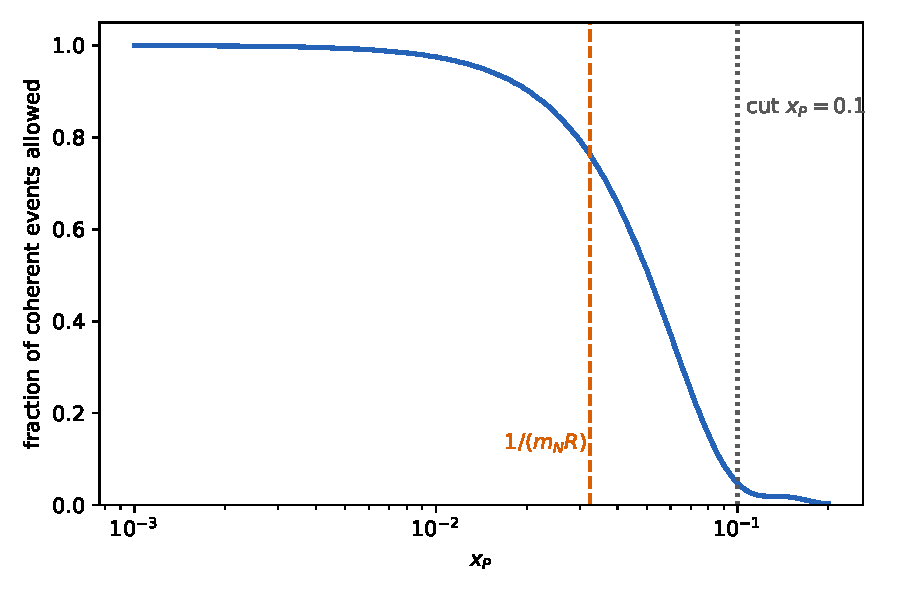
\includegraphics[width=0.7\linewidth]{coherent_tmin.pdf}
\end{center}

So the coherent cross section dies out between $x_{\mathbb P}\approx0.03$ and $0.1$. Above $0.1$
there are essentially no coherent events, and integrating to larger (or ``infinite'')
$x_{\mathbb P}$ would add nothing physical. (In any case $x_{\mathbb P}<1$ by kinematics.)

\section*{6. What this means for our calculation}

\begin{itemize}
\item Our diffractive formulas are derived in the small-$x$ (eikonal) limit, where $t_{\min}$ is
  neglected, i.e.\ the fraction above is set to 1. This is fine at small $x_{\mathbb P}$, but between
  $0.03$ and $0.1$ we \emph{overestimate} the coherent cross section.
\item Our dipole amplitude is also frozen above $x_{\mathbb P}=0.01$, and the small-$x$ framework
  is not meant for $x_{\mathbb P}\sim0.1$ or larger. Integrating further would add model
  artifacts, not physics.
\item Therefore $x_{\mathbb P}<0.1$ is a good, slightly generous, estimate of the full coherent
  contribution: the subtraction is, if anything, a bit too large, never too small.
\item It is also the same cut as in our diffractive predictions and in Guzey \textit{et al.}, so the
  subtracted piece is exactly what we show in the diffractive figures.
\end{itemize}

\section*{7. Possible sentence for the paper}

\begin{quote}\small
Since the $Xn$ selection removes all coherent events, the subtraction should in principle include
all $x_{\mathbb P}$. However, coherent scattering at large $x_{\mathbb P}$ is suppressed by the
nuclear form factor, since the minimum momentum transfer $|t_{\min}|\approx x_{\mathbb P}^2m_N^2$
exceeds $1/R^2$ for $x_{\mathbb P}\gtrsim0.03$. The cut $x_{\mathbb P}<0.1$ therefore includes
essentially the full coherent contribution.
\end{quote}

\section*{Appendix: derivation of $t_{\min}$}

We use light-cone coordinates, with the target moving in the minus direction, so that for any
four-vector
\begin{equation}
  k^2=2k^+k^--\mathbf k_\perp^2\,.
\end{equation}

\textbf{Incoming target.} Mass $m_N$, no transverse momentum. Being on shell, $2P^+P^-=m_N^2$, so
\begin{equation}
  P=\big(P^+,P^-,\mathbf P_\perp\big)=\Big(\frac{m_N^2}{2P^-},\;P^-,\;\mathbf 0\Big)\,.
\end{equation}

\textbf{Outgoing target.} By definition of $x_{\mathbb P}$ it keeps $(1-x_{\mathbb P})P^-$, it gets
a transverse kick $\boldsymbol\Delta$, and it stays on shell (it does not break up), which fixes
$P'^+=(m_N^2+\boldsymbol\Delta^2)/(2P'^-)$:
\begin{equation}
  P'=\Big(\frac{m_N^2+\boldsymbol\Delta^2}{2(1-x_{\mathbb P})P^-},\;(1-x_{\mathbb P})P^-,\;\boldsymbol\Delta\Big)\,.
\end{equation}

\textbf{Momentum transfer.} $k=P-P'$ has
\begin{align}
  k^- &= x_{\mathbb P}P^-\,,\\
  k^+ &= \frac{m_N^2}{2P^-}-\frac{m_N^2+\boldsymbol\Delta^2}{2(1-x_{\mathbb P})P^-}
       = -\frac{x_{\mathbb P}m_N^2+\boldsymbol\Delta^2}{2(1-x_{\mathbb P})P^-}\,,\\
  \mathbf k_\perp &= -\boldsymbol\Delta\,.
\end{align}

\textbf{Square it.}
\begin{align}
  t=2k^+k^--\boldsymbol\Delta^2
   &=-\frac{x_{\mathbb P}\big(x_{\mathbb P}m_N^2+\boldsymbol\Delta^2\big)}{1-x_{\mathbb P}}-\boldsymbol\Delta^2\nonumber\\
   &=-\frac{x_{\mathbb P}^2m_N^2+x_{\mathbb P}\boldsymbol\Delta^2+(1-x_{\mathbb P})\boldsymbol\Delta^2}{1-x_{\mathbb P}}\nonumber\\
   &=-\frac{\boldsymbol\Delta^2+x_{\mathbb P}^2m_N^2}{1-x_{\mathbb P}}\,.
\end{align}
The smallest $|t|$ is reached for $\boldsymbol\Delta=0$:
\begin{equation}
  |t_{\min}|=\frac{x_{\mathbb P}^2m_N^2}{1-x_{\mathbb P}}\approx x_{\mathbb P}^2m_N^2\,.
\end{equation}

\textbf{Physical meaning.} The target loses the large momentum $x_{\mathbb P}P^-$. To stay on
shell, its small component $P^+$ must change as well, by about $x_{\mathbb P}m_N^2/(2P^-)$. The
product $2k^+k^-\approx x_{\mathbb P}^2m_N^2$ does not depend on $P^-$: a larger collision energy
does not remove $t_{\min}$, only a smaller $x_{\mathbb P}$ does.

\textbf{For a nucleus.} We use $m_N$ per nucleon, since $x_{\mathbb P}$ is defined per nucleon.
With the nuclear mass $Am_N$ and the fraction per nucleus $x_{\mathbb P}/A$ the result is the same,
$(x_{\mathbb P}/A)^2(Am_N)^2=x_{\mathbb P}^2m_N^2$.

\end{document}
